\documentclass[twocolumn]{article}

\usepackage{scrextend}
\changefontsizes{8pt}

\makeatletter
\renewcommand*{\fps@figure}{!htb}
\renewcommand*{\fps@table}{!htb}
\makeatother

\usepackage{sectsty}
\sectionfont{\fontsize{11}{11}\selectfont}
\subsectionfont{\fontsize{10}{11}\selectfont}

\usepackage[compact]{titlesec}
\titlespacing{\section}{0pt}{2ex}{1ex}
\titlespacing{\subsection}{0pt}{1ex}{1ex}
\titlespacing{\subsubsection}{0pt}{0.5ex}{1ex}

\setlength{\parskip}{0cm}
\setlength{\parindent}{1em}

\usepackage{geometry}
 \geometry{
 a4paper,
 total={170mm,257mm},
 left=20mm,
 top=20mm,
 }
\usepackage[utf8]{inputenc}
\usepackage[hidelinks]{hyperref}
\usepackage{amsmath, bm}
\usepackage[ruled,vlined]{algorithm2e}
\usepackage{amssymb}
\usepackage{graphicx}
\usepackage{float}
\usepackage{booktabs}
\usepackage[parfill]{parskip}
\usepackage{comment}
\usepackage{subcaption}
\usepackage{booktabs}



\usepackage{listings}
\lstset{
    language=Python,
    breaklines=true,
    breakatwhitespace=true,
    basicstyle=\footnotesize,
    frame=lines
}
\usepackage[capitalise, nameinlink]{cleveref}

\usepackage[sorting=none, style=verbose]{biblatex}
\addbibresource{lab_6.bib}

\usepackage{titling}
\setlength{\droptitle}{-1cm}

\title{\Large COMP6248 Lab 6 Exercise -- Reflections on transfer learning}
\author{\small Wei Chien Teoh (Eugene)\\\bigskip \href{mailto:wct1c16@soton.ac.uk}{wct1c16@soton.ac.uk}}
\date{\small 29 April 2021}

\begin{document}

\maketitle

\section*{Introduction}

The results are seeded using \lstinline{pytorch_lightning.seed_everything(0)} to provide reproducible results.

\section{Transfer Learning}

\subsection{Finetuning}

In this section, a pretrained ResNet50 network is used as a backbone feature extractor, with frozen layers to prevent the weights from updating while training. A new Softmax classifier is used to replace the original dense layer. During the training phase, only the weights of the classifier were updated. The model in this section is denoted as Model 1. The justification of freezing the backbone layers is to prevent overfitting by training with the given small training dataset.

On top of the existing parameters stated in the lab sheet, a learning rate scheduler was used. The choice of learning rate scheduler for this model (Model 1) is the \lstinline{ReduceLROnPlateau} from PyTorch. \lstinline{ReduceLROnPlateau} is a dynamic scheduler which reduces the learning rate by a factor when a metric stops improving. In this model, the scheduler was set the the default parameters and used the training loss as the tracking metric. The model was trained for 50 epochs. The learning curves and learning rate plot is illustrated in \cref{fig:learning-curves}. The total training time for Model 1 is 13m 52s.

\cref{tab:model1-class-report} shows the classification performance for different classes. It is observed that despite the long training time, the model does not perform well on several classes. This is due to the unbalanced dataset provided.


\begin{figure}
    \centering
    \begin{subfigure}{.8\linewidth}
        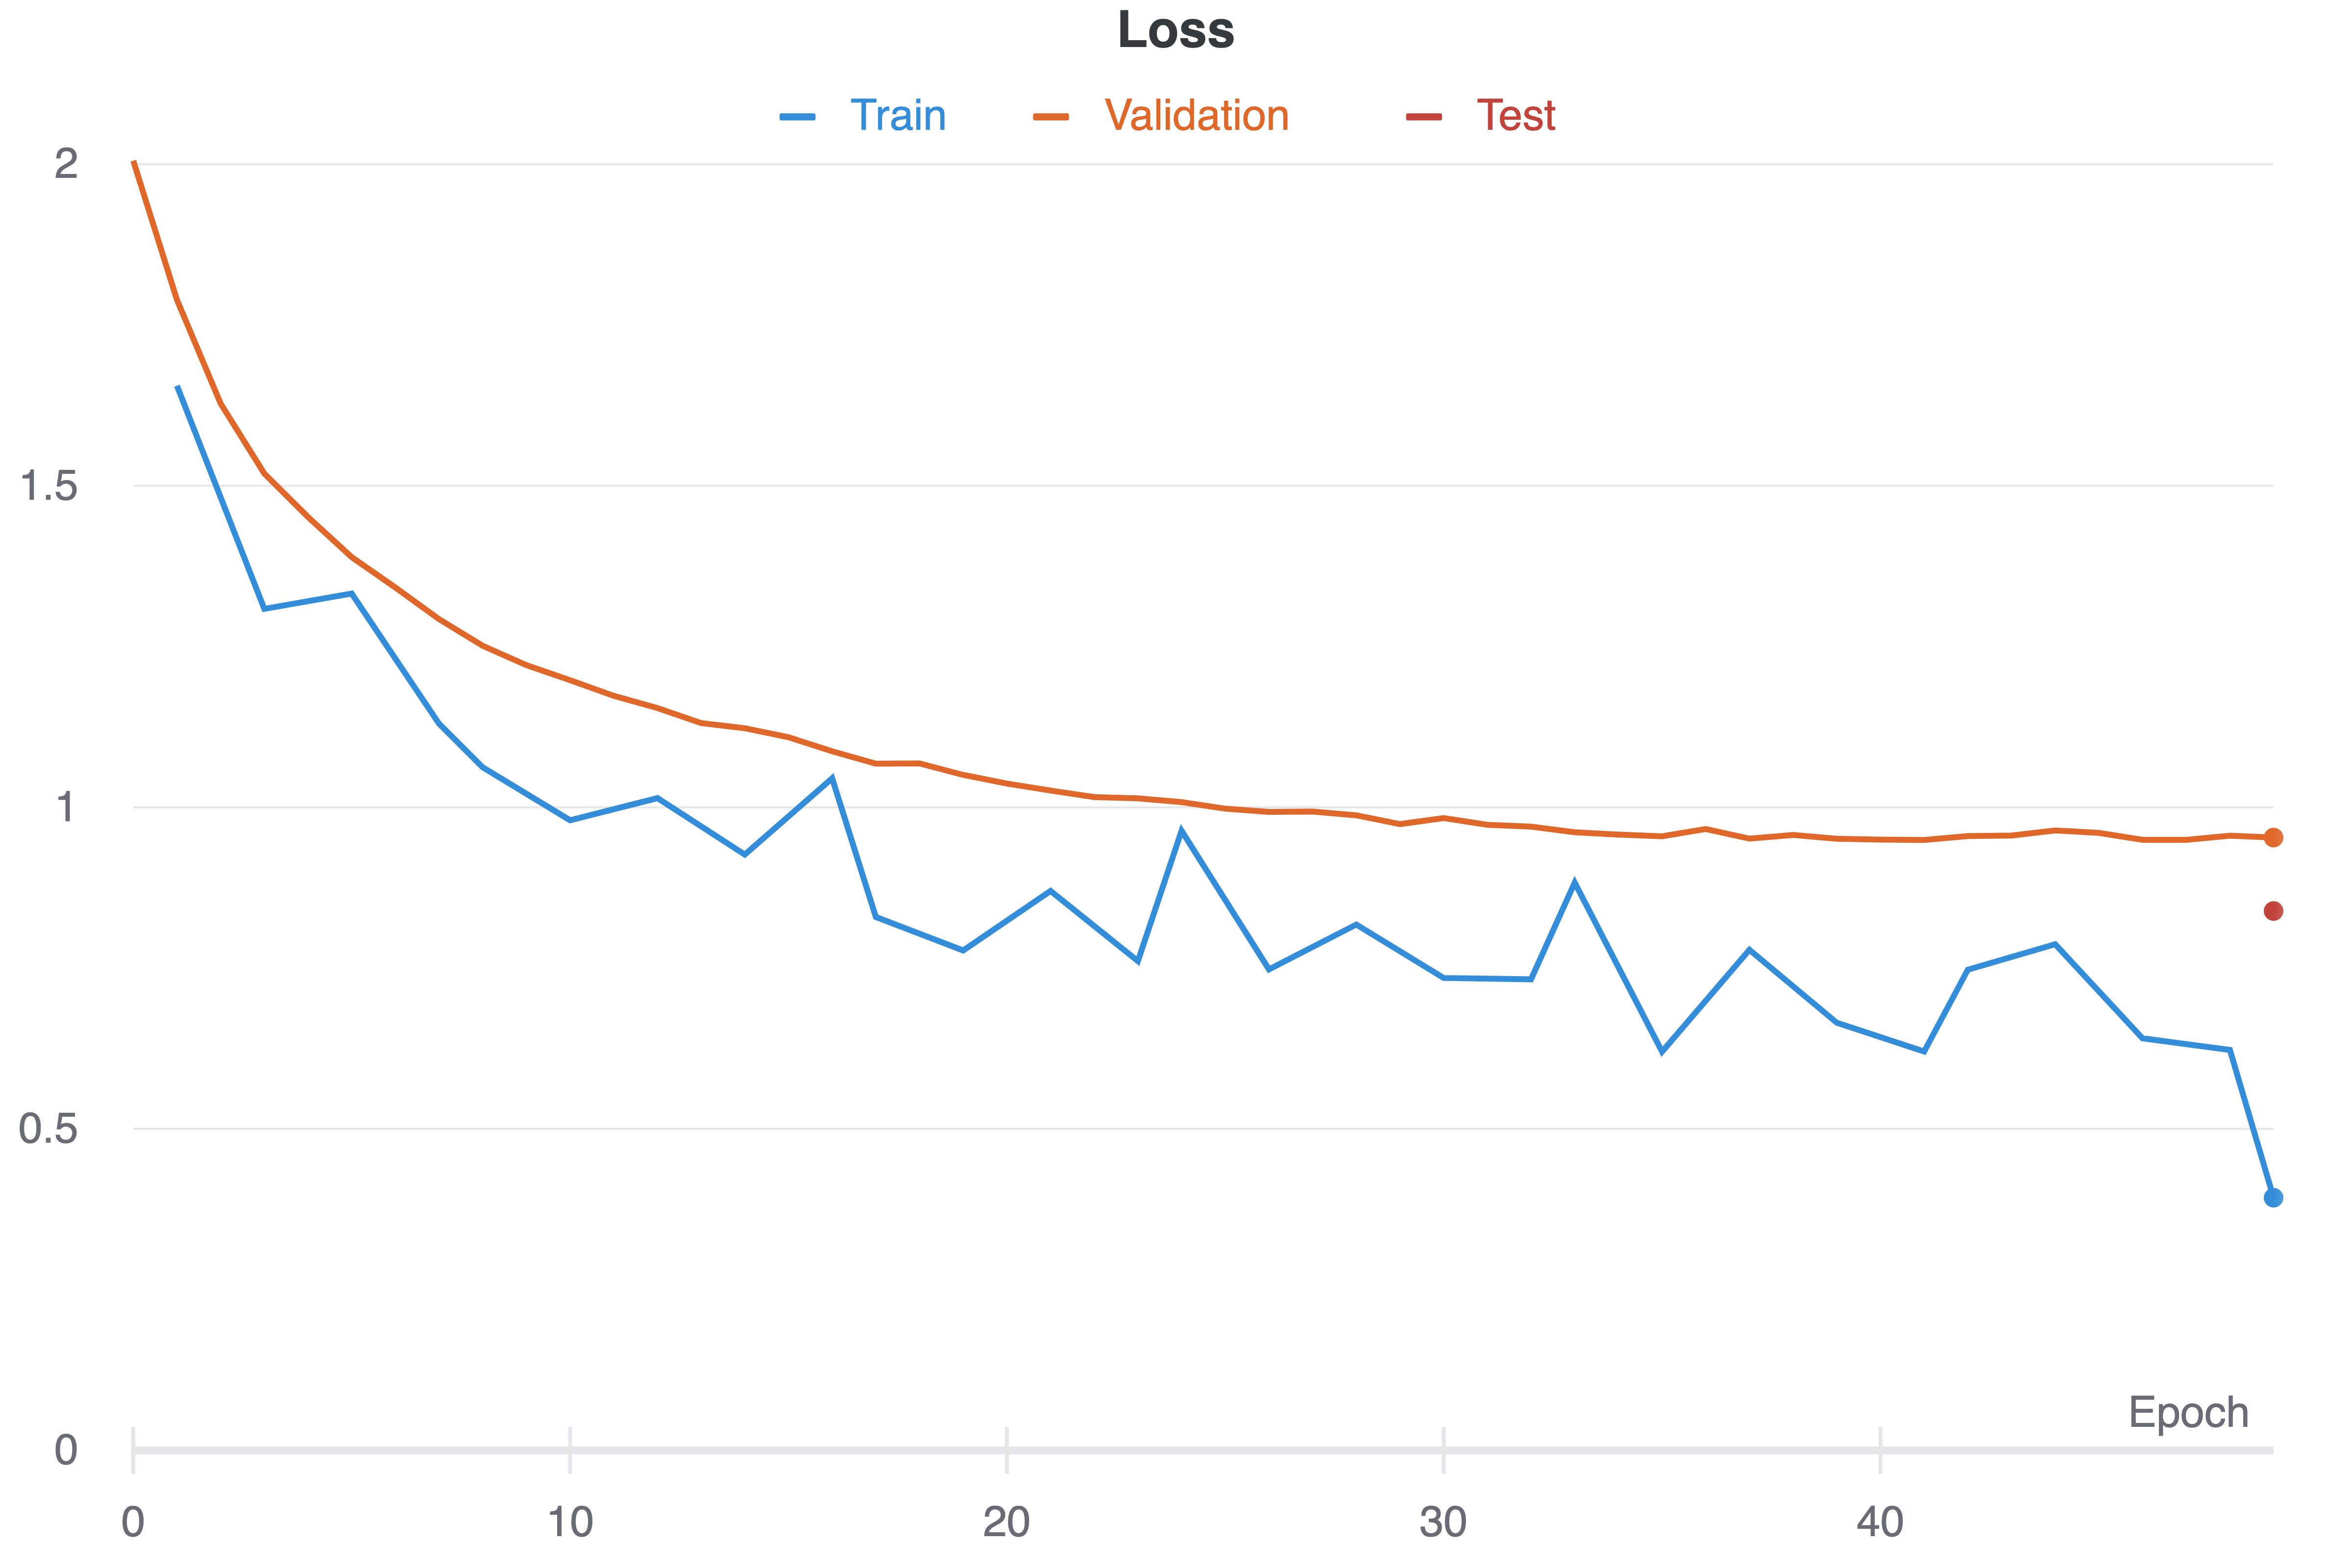
\includegraphics[width=\linewidth]{Figures/loss.png}
    \end{subfigure}
    \begin{subfigure}{.8\linewidth}
        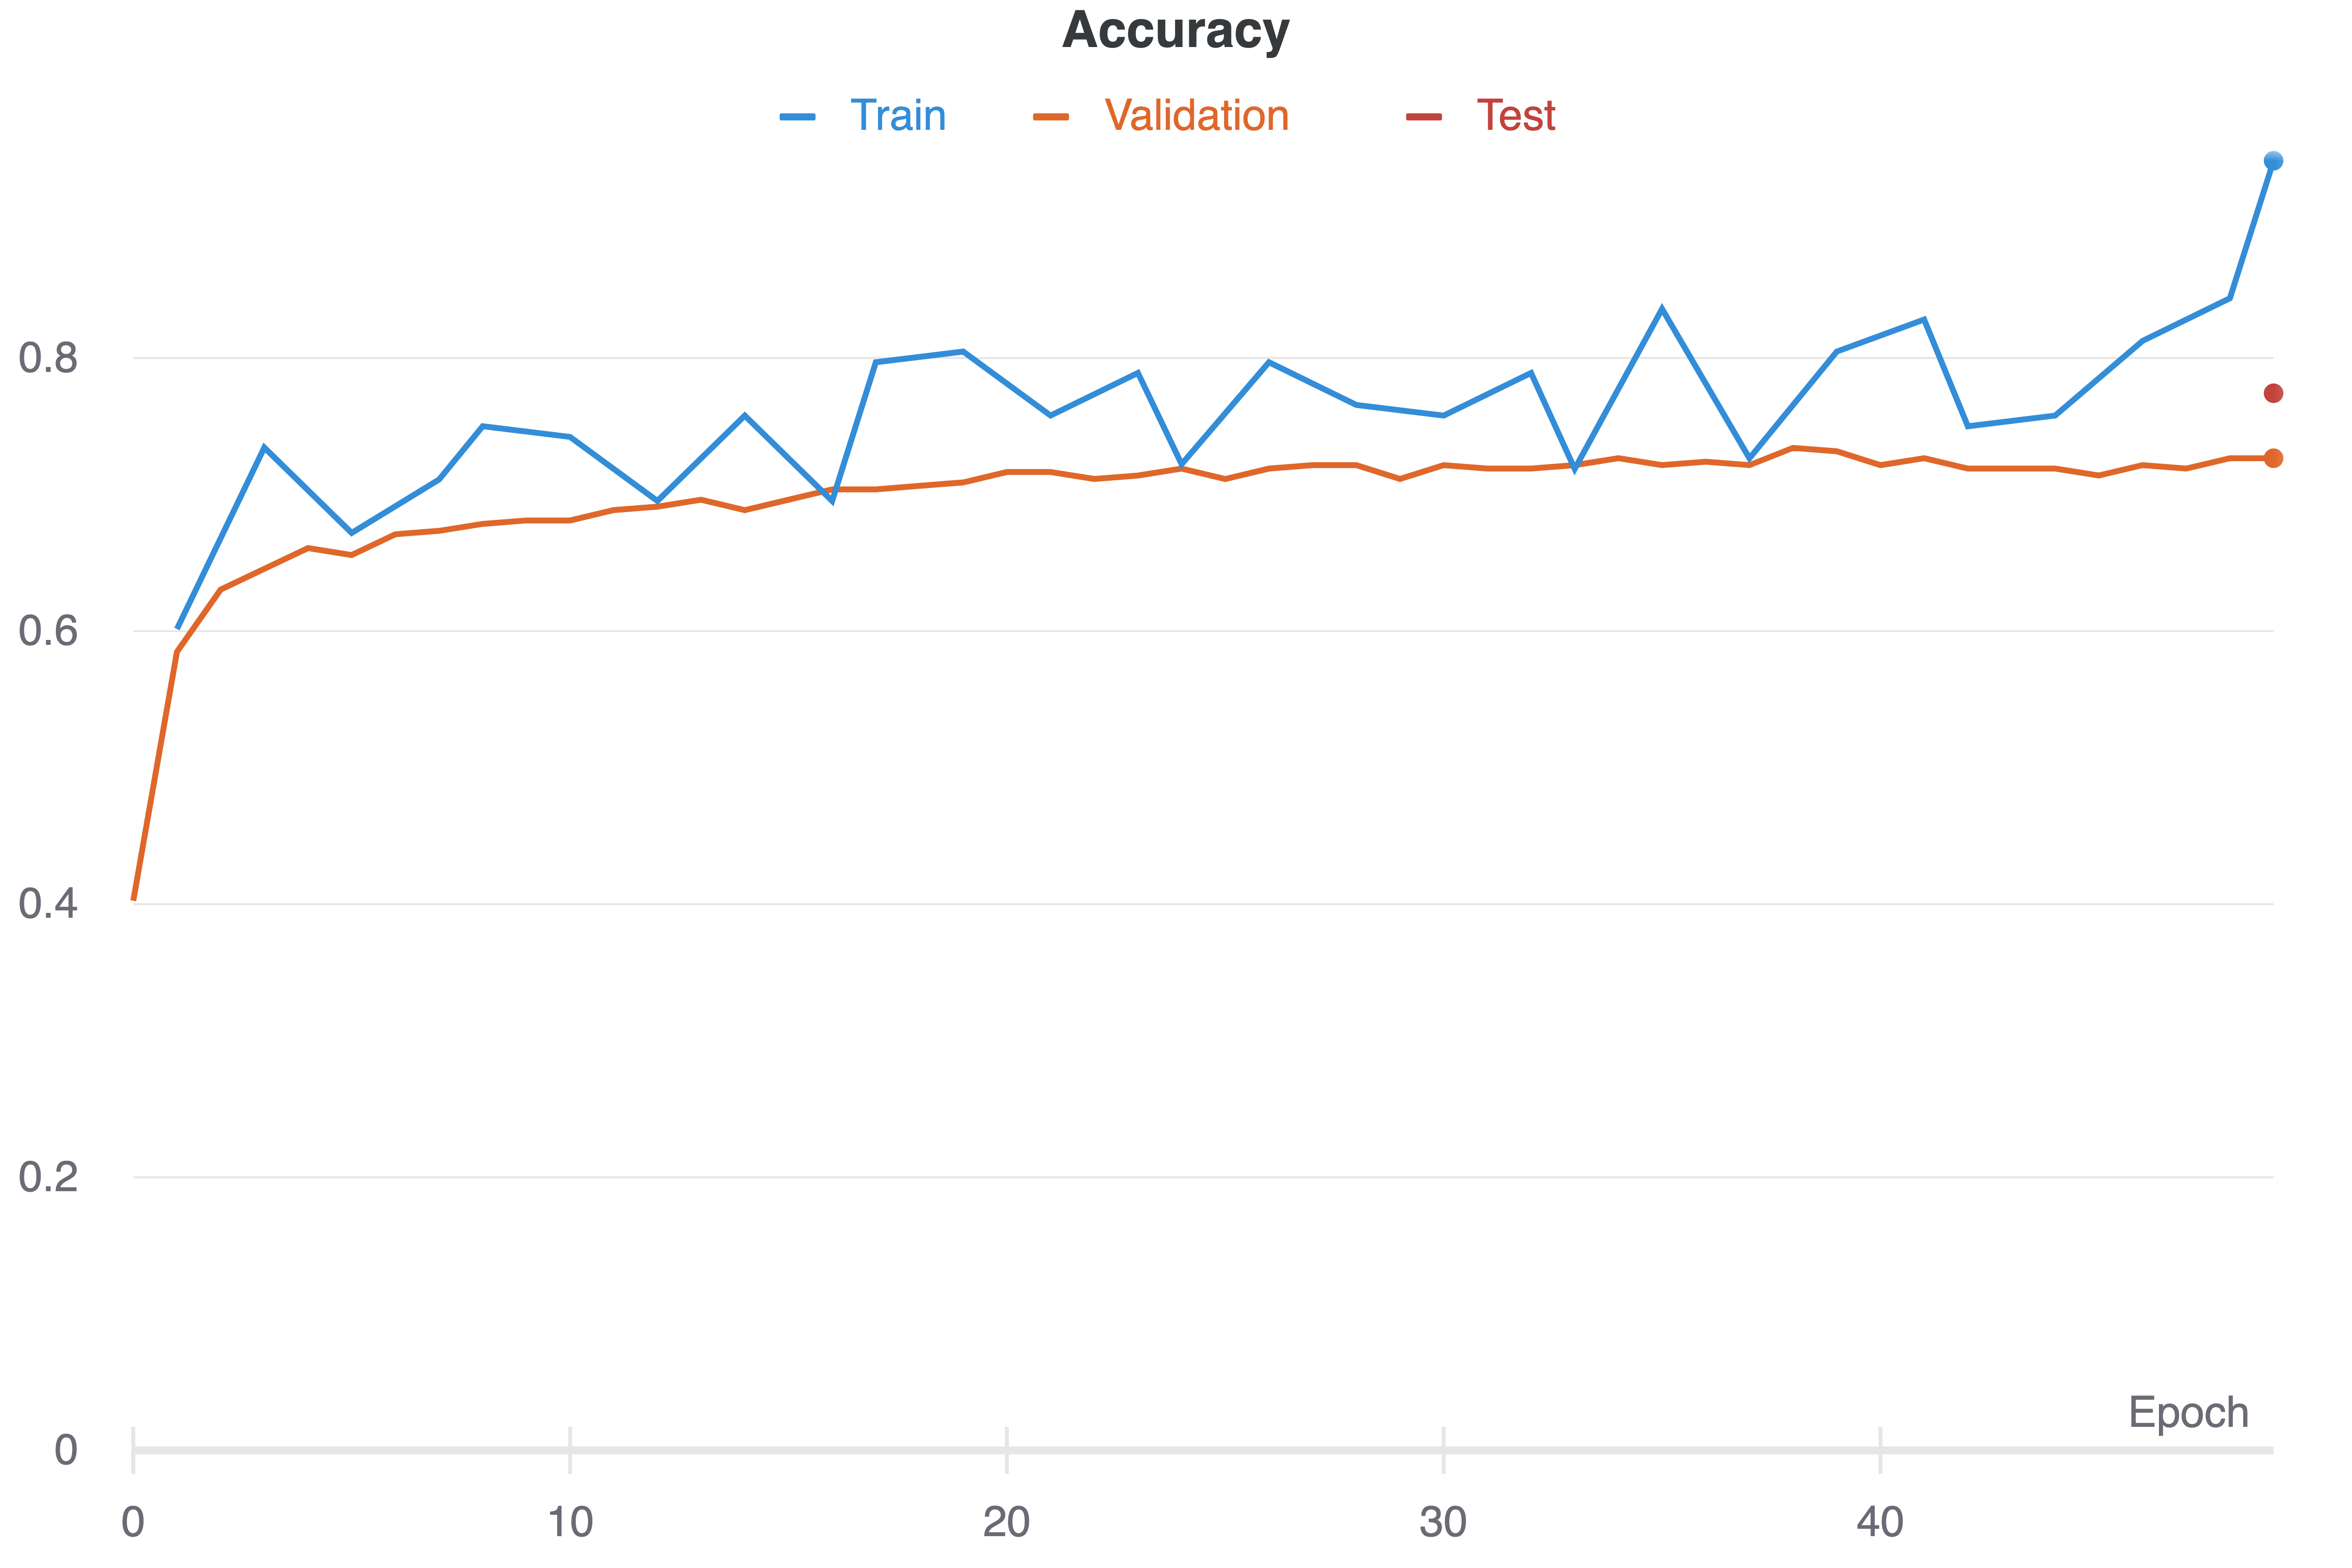
\includegraphics[width=\linewidth]{Figures/accuracy.png}
    \end{subfigure}
    \begin{subfigure}{.8\linewidth}
        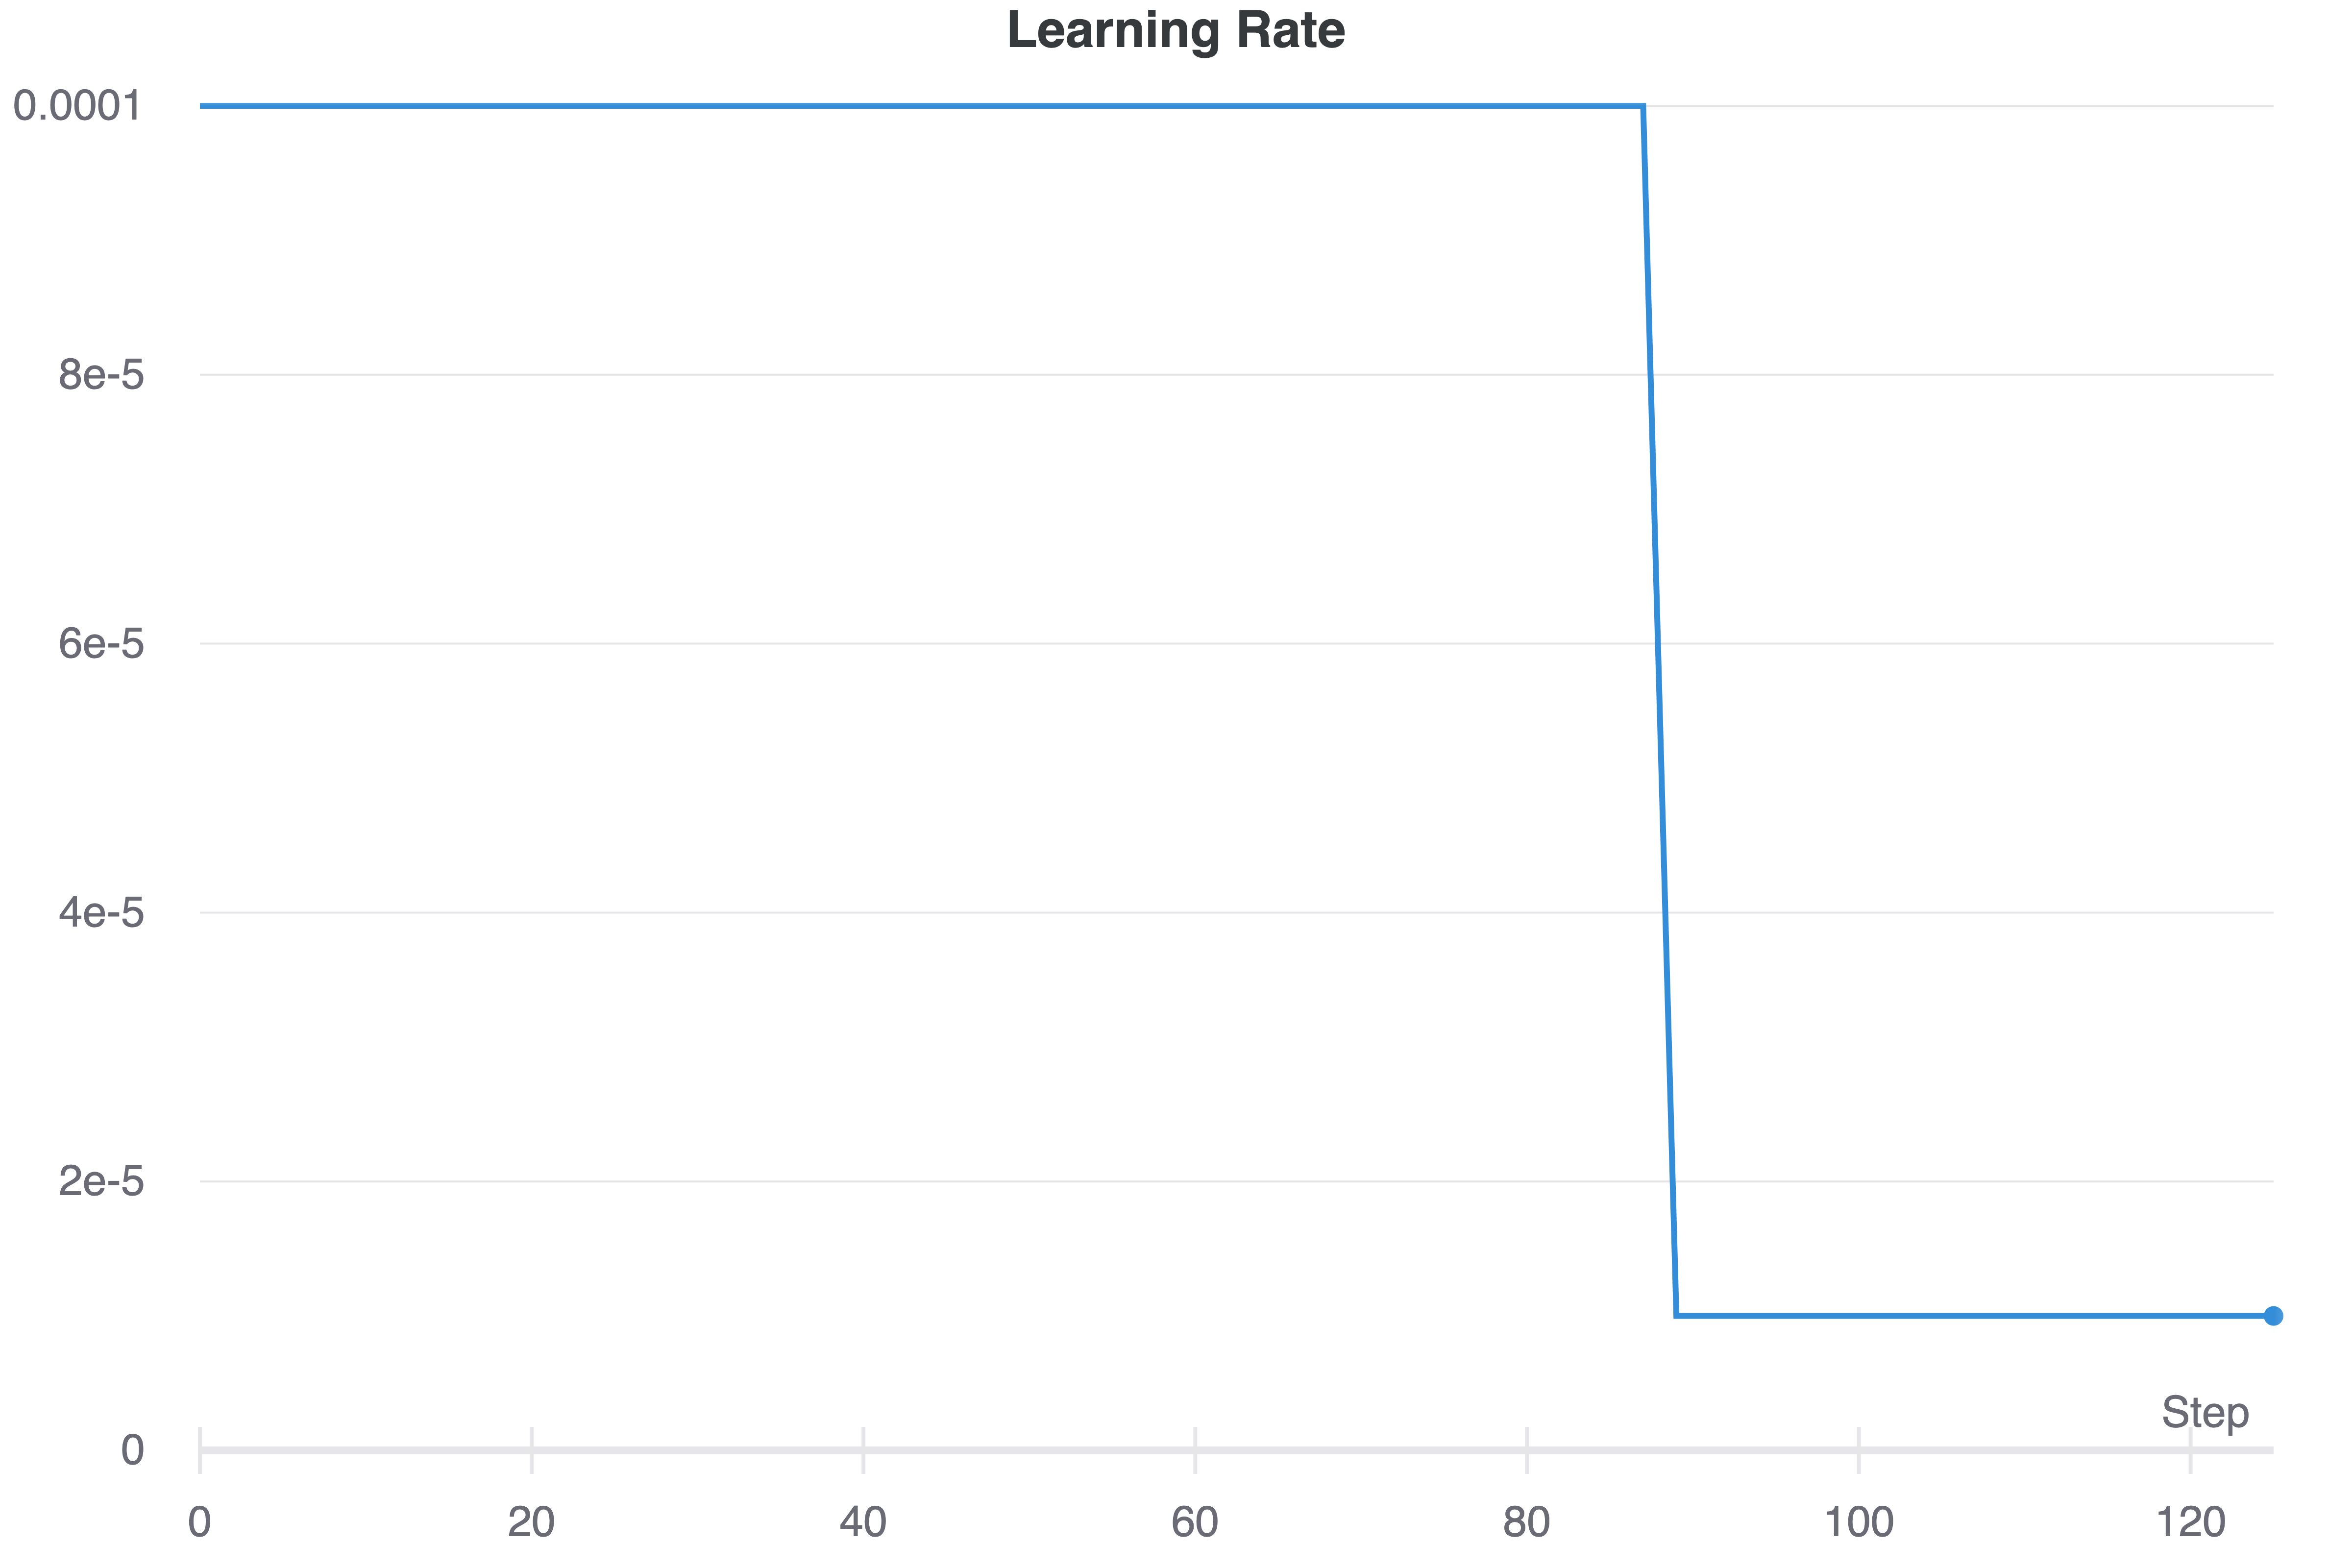
\includegraphics[width=\linewidth]{Figures/lr.png}
    \end{subfigure}
    \caption{Model 1 learning curves.}
    \label{fig:learning-curves}
\end{figure}

\begin{table}
    \centering
    \caption{Model 1 classification report.}
    \label{tab:model1-class-report}
    \begin{tabular}{lrrrr}
    \toprule
    class &  precision &  recall &  f1-score &   support \\
    \midrule
    0            &      0.412 &   0.368 &     0.389 &    19.000 \\
    1            &      0.556 &   0.455 &     0.500 &    22.000 \\
    2            &      0.636 &   0.137 &     0.226 &    51.000 \\
    3            &      0.000 &   0.000 &     0.000 &     3.000 \\
    4            &      0.000 &   0.000 &     0.000 &     7.000 \\
    5            &      0.179 &   0.085 &     0.115 &    59.000 \\
    6            &      0.667 &   0.667 &     0.667 &     3.000 \\
    7            &      0.000 &   0.000 &     0.000 &     1.000 \\
    8            &      0.672 &   0.861 &     0.755 &   274.000 \\
    9            &      0.367 &   0.541 &     0.437 &    74.000 \\
    10           &      1.000 &   0.067 &     0.125 &    15.000 \\
    11           &      0.647 &   0.579 &     0.611 &    19.000 \\
    12           &      0.000 &   0.000 &     0.000 &     3.000 \\
    13           &      0.000 &   0.000 &     0.000 &    29.000 \\
    14           &      0.964 &   0.997 &     0.980 &   325.000 \\
    15           &      0.926 &   0.948 &     0.936 &   420.000 \\
    accuracy     &      0.786 &   0.786 &     0.786 &     0.786 \\
    macro avg    &      0.439 &   0.356 &     0.359 &  1324.000 \\
    weighted avg &      0.760 &   0.786 &     0.758 &  1324.000 \\
    \bottomrule
    \end{tabular}
\end{table}


\subsection{Reflect on the two different approaches}

In this section, a Support Vector Machine (SVM) with Radial Basis Function (RBF) kernel is used to train on the feature extractor (or CNN code) of the ResNet50 network. The intuition behind this model is similar to that of Model 1, but with the Softmax classifier replaced with an SVM. The model in this section is denoted as Model 2. The total training time for Model 2 is 18s.

\cref{tab:model2-class-report} shows the classification performance for different classes. Model 2 significantly outperforms Model 1 in various classes as well as overall. It also required significantly less training time.

\begin{table}
    \centering
    \caption{Model 2 classification report.}
    \label{tab:model2-class-report}
    \begin{tabular}{lrrrr}
    \toprule
    class &  precision &  recall &  f1-score &   support \\
    \midrule
    0            &      0.905 &   1.000 &     0.950 &    19.000 \\
    1            &      0.818 &   0.818 &     0.818 &    22.000 \\
    2            &      0.765 &   0.255 &     0.382 &    51.000 \\
    3            &      1.000 &   0.667 &     0.800 &     3.000 \\
    4            &      0.000 &   0.000 &     0.000 &     7.000 \\
    5            &      0.818 &   0.305 &     0.444 &    59.000 \\
    6            &      1.000 &   1.000 &     1.000 &     3.000 \\
    7            &      0.000 &   0.000 &     0.000 &     1.000 \\
    8            &      0.818 &   0.985 &     0.894 &   274.000 \\
    9            &      0.411 &   0.838 &     0.551 &    74.000 \\
    10           &      0.667 &   0.133 &     0.222 &    15.000 \\
    11           &      1.000 &   0.737 &     0.848 &    19.000 \\
    12           &      0.000 &   0.000 &     0.000 &     3.000 \\
    13           &      0.000 &   0.000 &     0.000 &    29.000 \\
    14           &      0.991 &   1.000 &     0.995 &   325.000 \\
    15           &      0.993 &   0.971 &     0.982 &   420.000 \\
    accuracy     &      0.872 &   0.872 &     0.872 &     0.872 \\
    macro avg    &      0.637 &   0.544 &     0.556 &  1324.000 \\
    weighted avg &      0.869 &   0.872 &     0.852 &  1324.000 \\
    \bottomrule
    \end{tabular}
    \end{table}

% \begin{table}
%     \centering
%     \caption{Training time.}
%     \label{tab:runtime}
%     \begin{tabular}{ll}
%     \toprule
%     Model &  Runtime \\
%     \midrule
%     1 &    18.1s \\
%     2 &  13m 52s \\
%     \bottomrule
%     \end{tabular}
%     \end{table}


\end{document}